\documentclass[12pt, a4paper]{article}

\usepackage{listings}
\usepackage{color}
\usepackage{enumitem}
\usepackage{amsthm}
\usepackage{amssymb}
\usepackage{listings}
\usepackage{setspace}
\usepackage{graphicx}
\graphicspath{ {./figures/} }


\title{Deep Learning Fundamentals}
\author{William Darko}
\date{Summer 2021}

\pagenumbering{arabic}

\begin{document}

\maketitle
\newpage

\tableofcontents

\newpage

\section{About this course}
\paragraph*{}
Explore deep learning from scratch or broaden understanding of deep learning, via
practical hands-on code examples to solve concrete problems. We'll
utilise the Python language, and deep learning framework Keras with Tensor flow as a backend engine



\newpage

\section{Resources}

\begin{itemize}
   \item \textbf{Deep Learning with Python} (1st Edition) by François Chollet.
   Manning publisher
\end{itemize}

\newpage

\section{What is deep learning?}

\subsection{Artificial Intelligence}
{
   \centering
   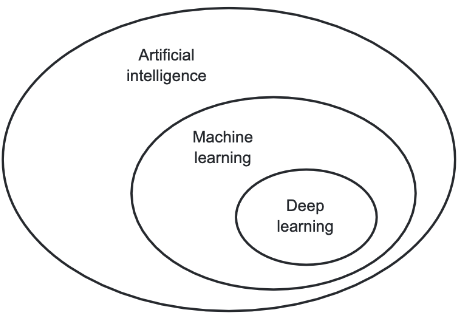
\includegraphics[width=8cm]{AI_Umbrella.png}

   the umbrella of Artificial intelligence

}

\paragraph*{}
We'll define Artificial intelligence to be the \textit{effort to automate intellectual 
tasks normally performed by humans.} AI is the general field that encompasses machine learning,
which deep learning is a subfield of.

\begin{itemize}
   \item Early AI took the approach of programmers manually implementing a large set of 
   rules for manupulating knowledge; this was known as \textbf{symbolic AI}.
   
   \item Symbolic AI turned out intractable, when applied to more complex problems like
   image classification, speech recogition, language translation, etc.
   
   \item Machine Learning was the new AI paradigm that rose to replace symbolic AI. It arises
   from the question: can computers go beyond what we tell it to do? How do computers learn
   on their own how to perform a specific task.
\end{itemize}

{
   \centering
   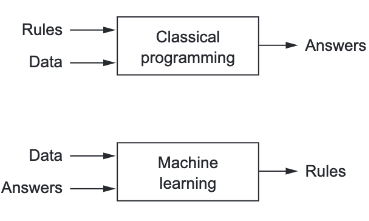
\includegraphics[width=6cm]{ML_new_paradigm.png}

    rules instead of answers in the ML paradigm

}

\begin{itemize}
   \item Recent AI trend driven by increase in computing power (faster hardware), and larger datasets.
\end{itemize}

\subsection{Learning representations from data}

\paragraph*{}
To do basic machine learning, three things are needed:
\begin{enumerate}
   \item \textbf{Input data} such as sound files, images, text documents, etc.
   \item \textbf{Examples of expected output} for training purposes
   \item \textbf{A way to measure the success of the algorithm} to determine the distance between
   algorithm's current output, and exptected output. 
\end{enumerate}

\textbf{The central problem in machine learning, and deep learning is to meaningfully transform data}.
Meaning, to learnin useful representations of the input data, which get us closer to the exptected output.
The learning aspect involves finding data transformations within an already defined set of operations
called the \textbf{hypothesis space}.


\subsection{The ``deep'' in deep learning}
\paragraph*{}
Deep learning as a subfield of machine learning, is a new take
on learning representations from data with emphasis on 
\textbf{learning successive leayers of increasingly meaningful representations}.

\begin{enumerate}
   \item How many layers contribute to a deep learning model of the data is called
   the \textbf{depth} of the model.
   \item Layered representations of data are almost always
   learned via models called \textbf{neural networks}.
   \item Think of deep neural networks as a multistage information-distillation
   operation, where information goes through successive filters (layers) and comes out
   increasingly purified.
   \item deep learning is essentially a multistage way to learn data representations.
\end{enumerate}
 
\subsection{Understanding how deep learning works}
\begin{enumerate}
   \item Deep neural networks conduct a mapping of inputs, to targets via deep sequence
   of data transformations.
   \item The specification of what a layer in a deep neural network does to its input data
   is stored in the layer's \textbf{weights}
   \item \textbf{Weights} of a layer are in essence, a ``bunch of numbers''
   \item The transformations implemented by a layer on its input data are \textbf{parameterised by its weights}.
   Thus weights are also called the \textbf{parameters of a layer}
   \item Initially, the weights of a network are randomised values.
   \item In a more detailed explanation, deep learning involves
   \textbf{finding a  set of values for the weights of all layers in a network
   such that the network will correctly map example inputs to their associated targets}
   \item To control the output of a neural network, we have to be able to measure how far its output is 
   from the output we desired. This is the job of the \textbf{loss/objective function}
   \item The \textbf{loss function} takes the predictions of a neural network, and the 
   desired prediction, and computes a distance score that captures \textbf{how well/accurate the network was on that specific example}
   \item The fundamental trick in deep learning is to use this distance score, the \textbf{loss score},
   to adjust the values of the weights in a direction that will lower the loss score,
   ultimately improving the accuracy of the network predictions.
   \item This adjustment of weights is the job of the \textbf{optimiser}, which
   implements a \textbf{Backpropagation algorithm}.
   \item A network with a minimal loss score is one which's outputs/predictions are 
   as close as possible to the desired/expected output; \textbf{a trained network}

   \item The \textbf{training loop} of a deep neural network:
   
   {
      \centering
      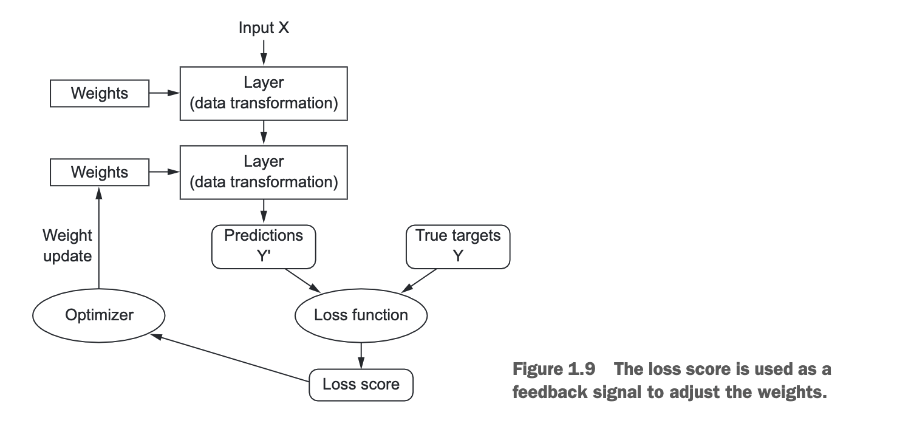
\includegraphics[width=12cm]{training_loop_dnn.png}

   }

   \textbf{Network layers parameterised by weights}, receive input data and \textbf{perform a sequence of
   meaningful data transformations picked from the hypothesis space}. The result of these transformations
   is an output prediction by the final layer, which is then passed to the loss function along with the
   desired output. The \textbf{loss function computes the loss score which is a distance of how far the networks prediction
   was from the ``correct" output}. This loss score is then utilised by the \textbf{optimiser which implements
   Backpropagation to adjust the weights of the layers in a direction that minimises the loss score}.

\end{enumerate}


\section{Building blocks of neural networks}
\subsection{Data representation of neural networks}
\begin{enumerate}
   \item \textbf{Scalars (0-Dimensional tensors)}: A tensor that contains one number,
   a scalar, of some numeric type. The number of dimensions/axes of tensor, also known in maths
   as the \textbf{rank}, can be found using the \textbf{ndim} attribtute provided by numpy.
   So for a scalar  \lstinline{x, x.ndim == 0}.
   \item \textbf{Vectors (1-Dimensional tensors)}: A tensor with one dimension, also known as a \textbf{vector},
   is simply an array of numbers. Keep in mind a vector, as a mathematical structure can be of an arbitrary
   number of dimensions. For instance, we can have a vector of rank 5; a 5-dimensional vector. Thus,
   a tensor rank is not the same as the rank of the vector. A vector is a 1-Dimensional tensor, but can be any number of dimensions
   as a vector.
   \item \textbf{Matrices (2D tensors)}: A matrix is a 2-dimensional tensor,
   but can be any arbitrary number of dimensions on row, and column axes of the matrix.
   Matrices are often implemented as an array of arrays; a 2-dimensional array, where
   the number of inner arrays are the number of dimensions on the rows axis, and the uniform length of the inner arrays,
   are the number of dimensions on the columns axis.
\end{enumerate}

\subsubsection{Key atrributes of tensors}
\begin{enumerate}
   \item \textbf{Number of axes (rank)}: For instance a matrix is a 2d-tensor, thus a rank of 2.
   A 3d tensor has a rank of 3. An n-dimensional tensor has a rank of n.
   \item \textbf{Shape}: Tuple of integers describing how many dimensions the tensor has
   on each axis. A scalar tensor has a shape of (); an empty shape tuple. A
   1-dimensional tensor, a vector, of an arbitrary k dimensions, will have a shape of (k,).
   A 2-dimensional tensor, a matrix, is of shape: (row, column) where row, and column are the
   number of dimensions on the row, and columns axes, respectively.
   \item \textbf{Data type}: The typeof data contained in the tensors.
   \item \textbf{Data batches}: the 0th axis of a tensor, is usually called the 
   \textbf{samples axis, or samples dimension}. The number of samples are usually split into 
   n equal parts, called batches. Nerual nets usually don't process an entire dataset at once; training of a neural net 
   is done in these data batches; partitions of the total number of samples.
\end{enumerate}


\subsubsection{Real-world examples of data tensors}
\paragraph*{}
Data in deep learning will almost always fall into one of these categories:
\begin{enumerate}
   \item \textbf{Vector data}: 2d tensors of shape \textbf{(samples, features)}
   \item \textbf{Timeseries data or sequence data}: 3d tensors of shape 
   (samples, timesteps, features)
   {
      \centering
      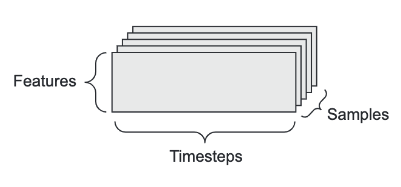
\includegraphics[width=10cm]{timeseries_data.png}

   }
   \item \textbf{Images}: 4d tensor of shape \textbf{(samples, height, width, channels)}
   or \textbf{(samples, channels, height, width)}. The shape for image data can follow the two
   most common conventions: \textbf{the colour channel first, or colour channel last convention}.
   {
      \centering
      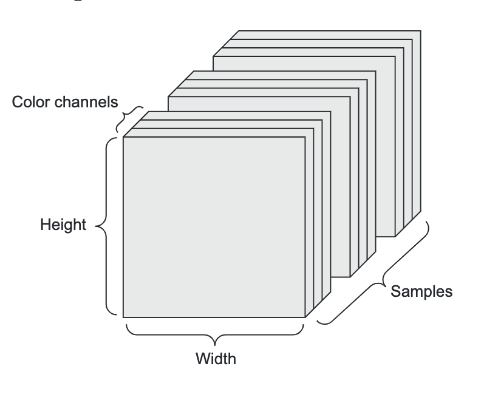
\includegraphics[width=8cm]{image_data.png}

   }
   \item \textbf{Video}: 5d tensors of shape \textbf{(samples, frames, height, width, channels)}
   or the colour channel first convention \textbf{(samples, channels, frames, height, width)}

\end{enumerate}

\section{Classification problems example}

\subsection{Binary classification}
\begin{enumerate}
   \item In binary classification problem (two output classes), network should
   end with dense layer on one hidden unit, and sigmoid activation
   \item Sequences of words can be encoded as binary vectors. Other encoding
   options can be used to fulfill the bit of preprocessing that needs to be done
   on the data before feeding it as tensors into the nerual network.
   \item Stacks of \textit{Dense} layers with with \textit{relu}
   activations can solve a wide range of sentiment analysis, and binary classification problems.
   \item When the output in binary classification is a scalar output like 1 or 0,
   the loss function to use is \textit{binary\_crossentropy}. 
   \textit{rmsprop} is generally a good enough optimiser for any classification problem.
\end{enumerate}

\subsection{Single-label multi-class classification}
\begin{enumerate}
   \item When trying to classify data points among \textit{N} classes,
   network should end with a \textit{Dense} layerof size \textit{N}.
   \item Network should end with a layer using \textit{softmax} activation
   so that it outputs a probability distribution across all N output classes.
   \item \textit{categorical\_crossentropy} is almost always the loss function used
   in single-label multi-class classification
   \item Ways to handle labels: either categorical/one-hot encoding, and using categorical crossentropy,
   or leave data as integers and use \textit{sparse\_categorical\_crossentropy}
   \item avoid information bottlenecks due to intermediate layers that are too small 
\end{enumerate}

\subsection{Regression}
\begin{enumerate}
   \item Loss function used in regression are different from that of other classification
   problems. \textbf{MSE (mean square error)} is the most common.
   \item Evaluation metrics are also different in regerssoin compared to other
   classification problem. \textbf{MAE (mean absolute error)} is the most common
   regression metric observed.
   \item Some preprocessing must me done on input data with values in varying 
   ranges. Each feature should be scaled independently as preprocessing step.
   \item When little data is available, using \textbf{K-fold} validation is a great
   way to reliably evaluate a model. K-fold validation involves dividing
   the data into K-partitions, and training on K-1 partitions while validation on the 
   remaining batch.
   \item Using smaller networks with fewer hidden layers is better when trying to avoid
   overfitting in the case that little training data is available. 
\end{enumerate}


\section{Four branches of machine learning}

\subsection{Supervised learning}
\begin{enumerate}
   \item consists of learning to map input ata to known targets called
   \textbf{annotations}
   \item some examples of supervised learning: classification,
   regression, sequence generation, syntax tree prediction,
   object detection, image segmentation.
\end{enumerate}

\subsection{Unsupervised}
\begin{enumerate}
   \item Consists of finding interesting transformation of input data without help
   of any targets.
   \item often a necessary step in better understanding dataset before attempting to solve
   a supervised learning problem.
   \item \textbf{Dimensionality reduction} and \textbf{clustering} are well-known categories of
   unsupervised learning.
\end{enumerate}

\subsection{Self-supervised learning}
\begin{enumerate}
   \item Supervised learning without the human annotated labels.
   \item Labels are still involved, but generated from input data typically using 
   a heuristic algorithm.
   \item \textbf{autoencoders} are well-known instance of self-supervised learning
   where generated targets are the input, but unmodified.
   \item Supervision in self-supervised learnign comes from future input data.
   \item For instance, predicting the next frame in a video clip giving previous frames, where
   the next frame in the input data is the target to map to, hence the supervision.
\end{enumerate}

\subsection{Reinforcement learning}
\begin{enumerate}
   \item involves an autonomous \textit{agent} receiving information about its
   environment, and learning to choose actions that maximise or minimise some metric
   or ``reward''.
\end{enumerate}

\subsection{Classification and regression glossary}
\begin{itemize}
   \item \textbf{Sample, or input}: Single data point that goes into your model
   \item \textbf{Prediction or output}: What is outputted by your model
   \item \textbf{Target}: the ground truth. What we desire our model to output
   \item \textbf{Prediction error or loss value}:  Measure of the distance between
   what model predicts, and the actual ground truth (the target)
   \item \textbf{Classes}: Set of possible labels to choose from in a classification problem
   \item \textbf{Label}: a specific instance of class annotation in classification problem. For
   instance if picture \#1056 is annotated as ``dog'', then ``dog'' is the label of
   picture \#1056.
   \item \textbf{Ground-truth annotations}: all targets for a dataset, collected, and labeled by humans
   \item \textbf{Binary classification}: Classification task where each input is mapped to one of two
   exclusive categories
   \item \textbf{Multi-class classification}: Classifiation task where inputs can be mapped
   to more than two categories. Outputs are usually a probability distribution over all categories.
   \item \textbf{Multi-label classification}: classification sample where each
   input sample can be mapped to multiple labels.
   \item \textbf{Scalar regression}: Task of mapping inputs to a target that is a 
   continuous scalar value.
   \item \textbf{Vector regression}: task of mapping inputs to 
   targets that are a set of continuous values.
   \item \textbf{Mini-batch or batch}: small set of smaples processed simultaneously
   by the model
\end{itemize}

\newpage
\section{Evaluating machine learning models}
\paragraph*{}
In machine learning, the central goal is to achieve \textbf{generalisation};
a model that performs well on data its never seen before. However, \textbf{overfitting},
is the central obstacle to this goal. Overfitting is when the perfomance of a model
degrades, and worsens on data its never seen before, compared to their perfomance
on training data.

There are several strategies for mitigating overfitting and maximising generalisation.
To measure generalisation, we look at ways to evaluate our machine learning models.

\begin{itemize}
   \item A part of machine learning involves tuning the \textbf{hyperparameters}
   of the model; hyperparameters such as the number of layers, or size of the layers.
   These hyperparameters are configured according to the networks performance on 
   validation data.
   \item \textbf{Information leaks, and overfitting to validation data}:
   after doing this step of tuning the network's hyperparameters according to perfomance
   on validation data, and then evaluating the network with that validation data,
   what begins to happen is that the \textbf{network starts to overfitt} to the validation data,
   and \textbf{some information about the validation data leaks into the model}.
   \item Since we care about generalisation, and not optimisation on the validation set,
   we should have a test data set completely separate from the validation set. The
   model should have no access to this set, not even indirectly.
\end{itemize}

\subsection{Splitting data into training, validation, and test sets}
\paragraph*{}
Methods such as \textbf{\textit{simple hold-out validation}, \textit{k-folds validation}, \textit{iterated
k-folds validation with shuffling}}.

\subsubsection{Simple hold-out validation}
\begin{enumerate}
   \item Set apart fraction of the data as test set, and use the remaining fraction
   as a training set.
   \item Because we want to prevent infromation leaks, we reserve a validation set as well,
   which we use as the validation set we tune our hyperparameters to.
   \item It's common to train the final model once again on both the training set,
   and validation set concatenated.
   \item It's also common to shuffle the entire available data before partitioning into training, and validation, and test set
   
   {
      \centering
      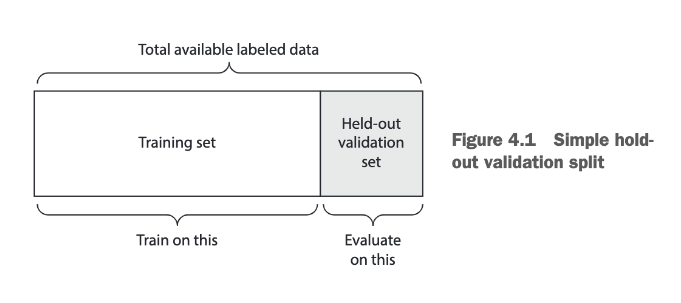
\includegraphics[width=12cm]{hold_out_validation.png}
      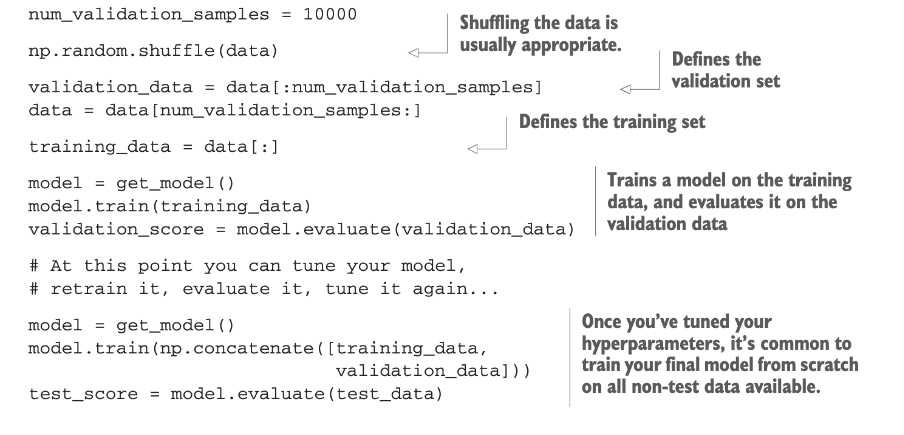
\includegraphics[width=12cm]{hold_out_validation_snippet.png}

   }
\end{enumerate}

\newpage
\subsubsection{K-fold validation}
\paragraph*{}
Simple hold-out validaion is only effective when there's ample amount of data to be 
partitioned into training, validation, and testing datasets. Thus, when little data 
is available, K-folds validation is an appropriate approach.

\begin{enumerate}
   \item Data is split into \textbf{\textit{K partitions}} of equal size.
   \item For \textbf{\textit{each partition i, train model on the remaining}}
   \textbf{\textit{K-1 partitions}} and \textbf{\textit{evaluate model on partition i}}
   \item Final validation score is the \textbf{averages of the K scores obtained}
   
   {
      \centering
      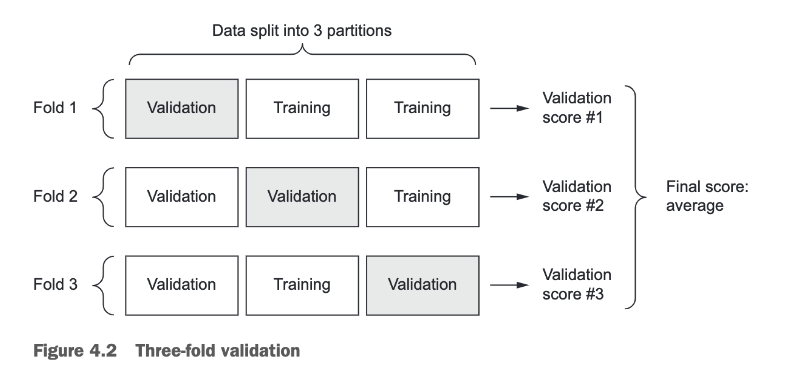
\includegraphics[width=10cm]{k_folds_validation_scheme.png}

      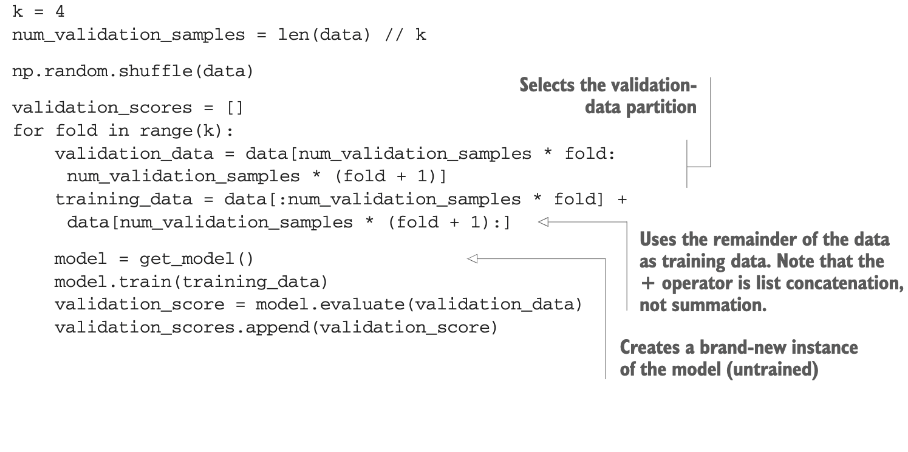
\includegraphics[width=12cm]{k_folds_validation_snip1.png}

      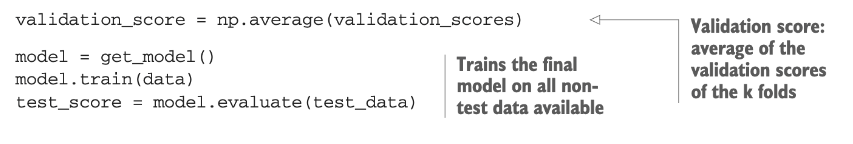
\includegraphics[width=12cm]{k_folds_validation_snip2.png}

   }
\end{enumerate}

\newpage
\subsubsection{Iterated K-folds validation with shuffling}
\begin{enumerate}
   \item Used when little data available, and need model evaluation as precise as possible 
   \item Involves applying K-folds validation multiple times (hence iterated k-folds),
   but shuffling the data each time before partitioning K-ways.
   \item Final score, similar to K-folds validation, is the average of scores from each iteration of 
   K-fold validation.
   \item Thus the model is trained and evaluated \textbf{\textit{P * K}} times,
   where \textbf{\textit{P}} is the number of iterations of K-folds validation.
\end{enumerate}


\subsection{Things to consider while choosing evaluation method}
\begin{enumerate}
   \item \textbf{Data representativeness}: To make sure the training and test sets,
   are representative of the data at hand, we want to avoid cases where we only train 
   on a subset of the classes of data available. For instance, when trying to classify 
   images of digits, and the dataset is soted by the classes of digits, simply taking a 
   subset of the dataset as it was, would mean only training the model on a set
   of only small class of numbers, effectively ignoring other digits. Hence, in this case,
   \textbf{randomly shuffling the data before creating any partitions} would allow there to be a diverse
   training data set.
   \item \textbf{The arrow of time}: If the task involves predicting the future,
   given past data such as predicting the next frame of a video, next word in a sentence,
   tomorrows weather given past weather data, randomly shuffling the data before 
   splitting into training, and testing sets, would create a \textbf{\textit{temporal leak}}.
   Meaning, model would effectively be trained on data from the future. 

   In such a situation, we should always ensure that test data is \textbf{\textit{posterior}}
   to data in the training set.

   \item \textbf{Redundancy in data}: If the entire dataset contains duplicate data points,
   which is quite common in real-world data, then its likely that both training, and test datasets would contain 
   common data points, hence we'll be testing, and evaluating our model on part of our training dataset,
   which is the worst thing that can happen!

   If the testing set includes training data, the model fails to generalise, and instead,
   optimises for the training data. Thus, its expedient to ensure that 
   training, and testing data are \textbf{disjoint}!
\end{enumerate}

\subsection{Preprocessing, feature engineering, and feature learning}
\paragraph*{}
The aim with preoprocessing is to make data more suitable for neural networks;
whether its via vectorisation, normalisation, or handling missing values, feature
extraction, raw data shouldn't be passed directly into nerual networks.

\subsubsection{Vectorisation}
\begin{enumerate}
   \item All inputs, and targets are made to be tensors of floating points,
   or in special cases, tensors of integers. 
   \item the preprocessing step of making all data into tensors is called 
   \textbf{\textit{data vectorisation}}. One example is using \textbf{one-hot-encoding}
\end{enumerate}

\subsubsection{Value Normalisation}
\begin{enumerate}
   \item Normaliing features independently so they have standard deviations of 1, and mean of 0
   \item Generally considered because its unsafe to feed neural networks data that take 
   relatively large values or heterogeneous data where data points take values in a different ranges.
   \item heterogeneous data should be normalised to acheive standard deviation of 1, and mean of 0 before
   fed into neural networks.
   \item normalisation is necessary to prevent large gradient updates that disallow network from converging.
   \item  Take small values; most values should be in range 0-1
   \item Data should be homogeneous; all features should take values in roughly the same range.
\end{enumerate}

\subsubsection{Handling missing values}
\begin{enumerate}
   \item When features aren't available for all samples, thus some samples are missing certain featuers,
   its often \textbf{safe to input missing values as 0}, with the condition that
   0 isn't a meaningful value in the dataset.
   \item Network will learn, and make the connection that \textbf{0 stands for missing value},
   and would start to ignore it altogether.
   \item Note that missing data has to be consistent across both the test dataset,
   and training dataset. If the network is trained on data with no missing data points,
   but features are missing in the test dataset, then the validation performace would be poor.
   One way to mitigate this is to artificially generate training samples with missing features consistent with that of 
   the test samples.
\end{enumerate}

\subsubsection{Feature engineering}
\begin{enumerate}
   \item Involves using your knowledge about the tast, the data at hand, and your knowledge of the machine learning algorithm,
   to \textbf{apply hardcoded transformations to the data before it goes into the model}.
   \item Data needs to present to the model in a way that makes learning easier.
\end{enumerate}

\section{Mitigating overfitting and  underfitting}
\paragraph*{}
Mitigating overfitting is essential to machine learning. Overfitting happens when 
our model degrades in performance when exposed to never before seen data. This is because 
the model started to memorise the training data, and learn irrelevant patterns, instead of 
trying to generalise.

The fundamental issue in machine learning is the tension between \textbf{optimisation} and \textbf{generalisation}.
\textbf{\textit{Optimisation} }refers to tuning our model's hyperparameters and architecture to attain the best perfomance possible.
While \textbf{\textit{generalisation}} refers to the model performing well on never before seen data.
The problem is, this optimisation step, may lead to the data overfitting to our validation set, or even training set after 
several epochs of training, and tuning.

Our model initially is \textbf{\textit{underfit}}; meaning there's still progress to be made. The network is yet to learn all the 
relevant parts of our training data. However as several iterations of training, and optimisation pass,
the network stops generalising, validation metrics begin to degrade and ultimately the model 
starts to overfit. It starts to \textbf{learn patterns specific to the training data, but misleading, and irrelevant to never before seend data}.

The best, and simplest way to mitigate overfitting is to simply get more 
training data to train the network. A network will naturally generalise the more 
training data its exposed to. However, if more training data isn't an option,
the next best thing is \textbf{\textit{regularisation}}.

\textbf{Regularisation} involves \textbf{modulating the quantity of information 
the model is allowed to store, or constraining what information the model 
should store}. The idea is that if the a network can only afford to memorise a 
small number of patterns, the \textbf{optimisation process froces the model to focus on 
the most prominent, hence, most important data patterns}. This offers a better chance 
of generalisation.

\subsubsection{Reducing size of the network}
\begin{enumerate}
   \item One of the simplest way to prevent overfitting is to reduce the size of the model;
   \textbf{the number of learnable parameters in the model, which are determined by the number of 
   layers, and the number of units per layer}
   \item The number of learnable parameters in a deep learning model, is often referred to 
   as the model's \textbf{\textit{capacity}}. A model with more parameters has 
   more \textbf{\textit{memorisation capacity}}
   \item A model with limited learning capacity would have to learn compressed 
   learning representations that have predictive  power regarding the targets, which is exactly the 
   type of representations we're interested in. 
   \item A compromise has to be found between \textbf{\textit{too much capacity}} and 
   \textbf{\textit{too little capacity}}
\end{enumerate}


\subsubsection{Adding weight regularisation}
\begin{enumerate}
   \item \textbf{\textit{Simple model}} is one where the distribution of parameter values has less entropy;
   thus one with fewer parameters.
   \item Common way to mitigate overfitting is to put contraints on the complexity of the network,
   by forcing the weights of the work to only take small values, making the weight distribution more 
   \textbf{\textit{regular}}.
   \item This technique of adding constraints to the complexity of the network is called 
   \textbf{\textit{weight regularisation}}. It involves \textbf{adding to the loss function, a cost associated with having large weights}.
   
\end{enumerate}


\end{document}